%%
%% Automatically generated file from DocOnce source
%% (https://github.com/hplgit/doconce/)
%%

% #define PREAMBLE

% #ifdef PREAMBLE
%-------------------- begin preamble ----------------------

\documentclass[%
oneside,                 % oneside: electronic viewing, twoside: printing
final,                   % draft: marks overfull hboxes, figures with paths
10pt,french]{article}

\listfiles               %  print all files needed to compile this document

\usepackage{relsize,makeidx,color,setspace,amsmath,amsfonts,amssymb}
\usepackage[table]{xcolor}
\usepackage{bm,ltablex,microtype}

\usepackage[pdftex]{graphicx}

% Packages for typesetting blocks of computer code
\usepackage{fancyvrb,framed,moreverb}

% Define colors
\definecolor{orange}{cmyk}{0,0.4,0.8,0.2}
\definecolor{tucorange}{rgb}{1.0,0.64,0}
\definecolor{darkorange}{rgb}{.71,0.21,0.01}
\definecolor{darkgreen}{rgb}{.12,.54,.11}
\definecolor{myteal}{rgb}{.26, .44, .56}
\definecolor{gray}{gray}{0.45}
\definecolor{mediumgray}{gray}{.8}
\definecolor{lightgray}{gray}{.95}
\definecolor{brown}{rgb}{0.54,0.27,0.07}
\definecolor{purple}{rgb}{0.5,0.0,0.5}
\definecolor{darkgray}{gray}{0.25}
\definecolor{darkblue}{rgb}{0,0.08,0.45}
\definecolor{darkblue2}{rgb}{0,0,0.8}
\definecolor{lightred}{rgb}{1.0,0.39,0.28}
\definecolor{lightgreen}{rgb}{0.48,0.99,0.0}
\definecolor{lightblue}{rgb}{0.53,0.81,0.92}
\definecolor{lightblue2}{rgb}{0.3,0.3,1.0}
\definecolor{lightpurple}{rgb}{0.87,0.63,0.87}
\definecolor{lightcyan}{rgb}{0.5,1.0,0.83}

\colorlet{comment_green}{green!50!black}
\colorlet{string_red}{red!60!black}
\colorlet{keyword_pink}{magenta!70!black}
\colorlet{indendifier_green}{green!70!white}

% Backgrounds for code
\definecolor{cbg_gray}{rgb}{.95, .95, .95}
\definecolor{bar_gray}{rgb}{.92, .92, .92}

\definecolor{cbg_yellowgray}{rgb}{.95, .95, .85}
\definecolor{bar_yellowgray}{rgb}{.95, .95, .65}

\colorlet{cbg_yellow2}{yellow!10}
\colorlet{bar_yellow2}{yellow!20}

\definecolor{cbg_yellow1}{rgb}{.98, .98, 0.8}
\definecolor{bar_yellow1}{rgb}{.98, .98, 0.4}

\definecolor{cbg_red1}{rgb}{1, 0.85, 0.85}
\definecolor{bar_red1}{rgb}{1, 0.75, 0.85}

\definecolor{cbg_blue1}{rgb}{0.87843, 0.95686, 1.0}
\definecolor{bar_blue1}{rgb}{0.7,     0.95686, 1}

%\setlength{\fboxsep}{-1.5mm}  % adjust cod_vpad/pro_vpad background box

%% Background for code blocks (parameter is color name)

%% pro/cod_vpad: gives some vertical padding before and after the text
%% (but has more simplistic code than _cod/pro_tight+cod/pro).
%% pro/cod_vpad can be used to enclose Verbatim or lst begin/end for code.
%% pro/cod calls _pro/cod_tight and has very little vertical padding,
%% used to enclose Verbatim and other begin/end for code.
%% (pro/cod is what the ptex2tex program could produce with the
%% Blue/BlueBar definitions in .ptex2tex.cfg.)

\newenvironment{cod_vpad}[1]{
   \def\FrameCommand{\colorbox{#1}}
   \MakeFramed{\FrameRestore}}
   {\endMakeFramed}

\newenvironment{_cod_tight}[1]{
   \def\FrameCommand{\colorbox{#1}}
   \FrameRule0.6pt\MakeFramed {\FrameRestore}\vskip3mm}
   {\vskip0mm\endMakeFramed}

\newenvironment{cod}[1]{
\bgroup\rmfamily
\fboxsep=0mm\relax
\begin{_cod_tight}{#1}
\list{}{\parsep=-2mm\parskip=0mm\topsep=0pt\leftmargin=2mm
\rightmargin=2\leftmargin\leftmargin=4pt\relax}
\item\relax}
{\endlist\end{_cod_tight}\egroup}

%% Background for complete program blocks (parameter 1 is color name
%% for background, parameter 2 is color for left bar)
\newenvironment{pro_vpad}[2]{
   \def\FrameCommand{\color{#2}\vrule width 1mm\normalcolor\colorbox{#1}}
   \MakeFramed{\FrameRestore}}
   {\endMakeFramed}

\newenvironment{_pro_tight}[2]{
   \def\FrameCommand{\color{#2}\vrule width 1mm\normalcolor\colorbox{#1}}
   \FrameRule0.6pt\MakeFramed {\advance\hsize-2mm\FrameRestore}\vskip3mm}
   {\vskip0mm\endMakeFramed}

\newenvironment{pro}[2]{
\bgroup\rmfamily
\fboxsep=0mm\relax
\begin{_pro_tight}{#1}{#2}
\list{}{\parsep=-2mm\parskip=0mm\topsep=0pt\leftmargin=2mm
\rightmargin=2\leftmargin\leftmargin=4pt\relax}
\item\relax}
{\endlist\end{_pro_tight}\egroup}

\usepackage{minted}
\usemintedstyle{default}

\usepackage[T1]{fontenc}
%\usepackage[latin1]{inputenc}
\usepackage{ucs}
\usepackage[utf8x]{inputenc}

\usepackage{lmodern}         % Latin Modern fonts derived from Computer Modern

% Hyperlinks in PDF:
\definecolor{linkcolor}{rgb}{0,0,0.4}
\usepackage{hyperref}
\hypersetup{
    breaklinks=true,
    colorlinks=true,
    linkcolor=linkcolor,
    urlcolor=linkcolor,
    citecolor=black,
    filecolor=black,
    %filecolor=blue,
    pdfmenubar=true,
    pdftoolbar=true,
    bookmarksdepth=3   % Uncomment (and tweak) for PDF bookmarks with more levels than the TOC
    }
%\hyperbaseurl{}   % hyperlinks are relative to this root

\setcounter{tocdepth}{2}  % levels in table of contents

% Tricks for having figures close to where they are defined:
% 1. define less restrictive rules for where to put figures
\setcounter{topnumber}{2}
\setcounter{bottomnumber}{2}
\setcounter{totalnumber}{4}
\renewcommand{\topfraction}{0.95}
\renewcommand{\bottomfraction}{0.95}
\renewcommand{\textfraction}{0}
\renewcommand{\floatpagefraction}{0.75}
% floatpagefraction must always be less than topfraction!
% 2. ensure all figures are flushed before next section
\usepackage[section]{placeins}
% 3. enable begin{figure}[H] (often leads to ugly pagebreaks)
%\usepackage{float}\restylefloat{figure}

% --- fancyhdr package for fancy headers ---
\usepackage{fancyhdr}
\fancyhf{} % sets both header and footer to nothing
\renewcommand{\headrulewidth}{0pt}
\fancyfoot[LE,RO]{\thepage}
% Ensure copyright on titlepage (article style) and chapter pages (book style)
\fancypagestyle{plain}{
  \fancyhf{}
  \fancyfoot[C]{{\footnotesize \copyright\ 2019, Ahmed Ammar. Released under CC Attribution 4.0 license}}
%  \renewcommand{\footrulewidth}{0mm}
  \renewcommand{\headrulewidth}{0mm}
}
% Ensure copyright on titlepages with \thispagestyle{empty}
\fancypagestyle{empty}{
  \fancyhf{}
  \fancyfoot[C]{{\footnotesize \copyright\ 2019, Ahmed Ammar. Released under CC Attribution 4.0 license}}
  \renewcommand{\footrulewidth}{0mm}
  \renewcommand{\headrulewidth}{0mm}
}

\pagestyle{fancy}


\usepackage{framed,wrapfig}

% --- begin definitions of admonition environments ---

% Admonition style "grayicon" has colored background, no frame, and an icon
% Admon "notice"
\definecolor{grayicon_notice_background}{rgb}{0.91,0.91,0.91}
% \fboxsep sets the space between the text and the box
\newenvironment{noticeshaded}
{\def\FrameCommand{\fboxsep=3mm\colorbox{grayicon_notice_background}}
 \MakeFramed {\advance\hsize-\width \FrameRestore}}{\endMakeFramed}

\newenvironment{notice_grayiconadmon}[1][Notice]{
\begin{noticeshaded}
\noindent
\begin{wrapfigure}{l}{0.07\textwidth}
\vspace{-13pt}

\includegraphics[width=0.07\textwidth]{latex_figs/small_gray_notice}
\end{wrapfigure} \textbf{#1}\par
\nobreak\noindent\ignorespaces
}
{
\end{noticeshaded}
}

% Admonition style "grayicon" has colored background, no frame, and an icon
% Admon "summary"
\definecolor{grayicon_summary_background}{rgb}{0.91,0.91,0.91}
% \fboxsep sets the space between the text and the box
\newenvironment{summaryshaded}
{\def\FrameCommand{\fboxsep=3mm\colorbox{grayicon_summary_background}}
 \MakeFramed {\advance\hsize-\width \FrameRestore}}{\endMakeFramed}

\newenvironment{summary_grayiconadmon}[1][Summary]{
\begin{summaryshaded}
\noindent
\begin{wrapfigure}{l}{0.07\textwidth}
\vspace{-13pt}
\includegraphics[width=0.07\textwidth]{latex_figs/small_gray_summary}
\end{wrapfigure} \textbf{#1}\par
\nobreak\noindent\ignorespaces
}
{
\end{summaryshaded}
}

% Admonition style "grayicon" has colored background, no frame, and an icon
% Admon "warning"
\definecolor{grayicon_warning_background}{rgb}{0.91,0.91,0.91}
% \fboxsep sets the space between the text and the box
\newenvironment{warningshaded}
{\def\FrameCommand{\fboxsep=3mm\colorbox{grayicon_warning_background}}
 \MakeFramed {\advance\hsize-\width \FrameRestore}}{\endMakeFramed}

\newenvironment{warning_grayiconadmon}[1][Warning]{
\begin{warningshaded}
\noindent
\begin{wrapfigure}{l}{0.07\textwidth}
\vspace{-13pt}
\includegraphics[width=0.07\textwidth]{latex_figs/small_gray_warning}
\end{wrapfigure} \textbf{#1}\par
\nobreak\noindent\ignorespaces
}
{
\end{warningshaded}
}

% Admonition style "grayicon" has colored background, no frame, and an icon
% Admon "question"
\definecolor{grayicon_question_background}{rgb}{0.91,0.91,0.91}
% \fboxsep sets the space between the text and the box
\newenvironment{questionshaded}
{\def\FrameCommand{\fboxsep=3mm\colorbox{grayicon_question_background}}
 \MakeFramed {\advance\hsize-\width \FrameRestore}}{\endMakeFramed}

\newenvironment{question_grayiconadmon}[1][Question]{
\begin{questionshaded}
\noindent
\begin{wrapfigure}{l}{0.07\textwidth}
\vspace{-13pt}
\includegraphics[width=0.07\textwidth]{latex_figs/small_gray_question2}
\end{wrapfigure} \textbf{#1}\par
\nobreak\noindent\ignorespaces
}
{
\end{questionshaded}
}

% Admonition style "grayicon" has colored background, no frame, and an icon
% Admon "block"
\definecolor{grayicon_block_background}{rgb}{0.91,0.91,0.91}
% \fboxsep sets the space between the text and the box
\newenvironment{blockshaded}
{\def\FrameCommand{\fboxsep=3mm\colorbox{grayicon_block_background}}
 \MakeFramed {\advance\hsize-\width \FrameRestore}}{\endMakeFramed}

\newenvironment{block_grayiconadmon}[1][Block]{
\begin{blockshaded}
\noindent
 \textbf{#1}\par
\nobreak\noindent\ignorespaces
}
{
\end{blockshaded}
}

% --- end of definitions of admonition environments ---

% prevent orhpans and widows
\clubpenalty = 10000
\widowpenalty = 10000

% --- end of standard preamble for documents ---


\usepackage[french]{babel}

% insert custom LaTeX commands...

\raggedbottom
\makeindex
\usepackage[totoc]{idxlayout}   % for index in the toc
\usepackage[nottoc]{tocbibind}  % for references/bibliography in the toc

%-------------------- end preamble ----------------------

\begin{document}

% matching end for #ifdef PREAMBLE
% #endif

\newcommand{\exercisesection}[1]{\subsection*{#1}}


% ------------------- main content ----------------------



% ----------------- title -------------------------

\title{Introduction à Python pour les ingénieurs}

% ----------------- author(s) -------------------------

\author{Ahmed Ammar\footnote{Email: \texttt{ahmed.ammar@fst.utm.tn}. Faculté des Sciences de Tunis, Université de Tunis El Manar.}}

% ----------------- end author(s) -------------------------

\date{Feb 7, 2019}
\maketitle

\tableofcontents


\vspace{1cm} % after toc




% !split
\section{Introduction}

Python (\href{{http://www.python.org/}}{\nolinkurl{http://www.python.org/}}) est un langage de programmation moderne de haut niveau, orienté objet et d'usage général.

\textbf{Caractéristiques générales de Python} :

\begin{itemize}
\item Langage simple:
\begin{itemize}

  \item facile à lire et à apprendre avec une syntaxe minimaliste.

\end{itemize}

\noindent
\item Langage concis et expressif:
\begin{itemize}

  \item moins de lignes de code

  \item moins de bugs

  \item plus facile à maintenir.
\end{itemize}

\noindent
\end{itemize}

\noindent
\textbf{Détails techniques} :

\begin{itemize}
\item Typé dynamiquement:
\begin{itemize}

  \item Pas besoin de définir le type des variables, les arguments ou le type des fonctions.

\end{itemize}

\noindent
\item La gestion automatique de la mémoire:
\begin{itemize}

  \item Aucune nécessité d'allouer explicitement et désallouer la mémoire pour les variables et les tableaux de données. Aucun bug de fuite de mémoire.

\end{itemize}

\noindent
\item Interprété:
\begin{itemize}

  \item Pas besoin de compiler le code. L'interpréteur Python lit et exécute le code python directement.
\end{itemize}

\noindent
\end{itemize}

\noindent
\textbf{Avantages} :

\begin{itemize}
\item Le principal avantage est la facilité de programmation, qui minimise le temps nécessaire pour développer, déboguer et maintenir le code.

\item Langage bien conçu qui encourage les bonnes pratiques de programmation:
\begin{itemize}

  \item Modulaire et orientée objet, permet l'encapsulation  et la réutilisation de code. Il en résulte souvent un code plus transparent, plus facile à améliorer et sans bug.

  \item Documentation intégré avec le code.

\end{itemize}

\noindent
\item De nombreuses bibliothèques standards, et de nombreux packages add-on.
\end{itemize}

\noindent
% !split
\section{Avoir Python installé sur sa machine}
L’installation d’un environnement Python complet peut-être une vraie galère. Déjà, il faut télécharger Python et l’installer. Par la suite, télécharger un à un les packages dont on a besoin. Parfois, le nombre de ces librairies peut-être grand.

Par ailleurs, il faut s’assurer L’installation d’un environnement Python complet peut-être une vraie galère. Déjà, il faut télécharger Python et l’installer. Par la suite, télécharger un à un les packages dont on a besoin. Parfois, le nombre de ces librairies peut-être grand.

Par ailleurs, il faut s’assurer de la compatibilité entre les versions des différentes packages qu’on a à télécharger.

Bref, ce n’est pas amusant!


\subsection{Distribution Anaconda}
Nous demandons à tous les étudiants de télécharger Anaconda. Pour cela, il faut télécharger un installeur à partir de \href{{https://www.anaconda.com/download/}}{\nolinkurl{https://www.anaconda.com/download/}}, correspondant à votre système d’exploitation (Windows, Mac OS X, Linux). Il faut choisir entre 32 bits ou 64 bits (pour la version \emph{Python 3}) selon que votre système d’exploitation est 32 bits ou 64 bits.

\subsection{Comment démarrer le navigateur Anaconda?}
Lorsque vous installez \textbf{Anaconda} sous Windows, Linux ou macOS, une icône est automatiquement ajoutée au menu de votre programme et/ou à votre bureau pour lancer \textbf{Anaconda Navigator}.
Vous pouvez également lancer Anaconda Navigator à partir d'une invite de commande Windows ou d'un terminal ubuntu  à l'aide de la commande suivante:
\begin{cod}{cbg_gray}\begin{minted}[fontsize=\fontsize{9pt}{9pt},linenos=false,baselinestretch=1.0,fontfamily=tt,xleftmargin=2mm]{text}
$ anaconda-navigator
\end{minted}
\end{cod}
\noindent

Différentes distributions Linux telles que \emph{CentOS} ou \emph{Ubuntu} ont de nombreux systèmes permettant d’ajouter des raccourcis aux menus et au bureau. Anaconda n’ajoute donc pas ces raccourcis automatiquement. À la place, vous pouvez utiliser votre système d'exploitation pour créer des raccourcis qui exécutent la commande \texttt{anaconda-navigator} sur le bureau ou dans le menu principal du système d'exploitation, ou les deux.


\begin{figure}[!ht]  % 
  \centerline{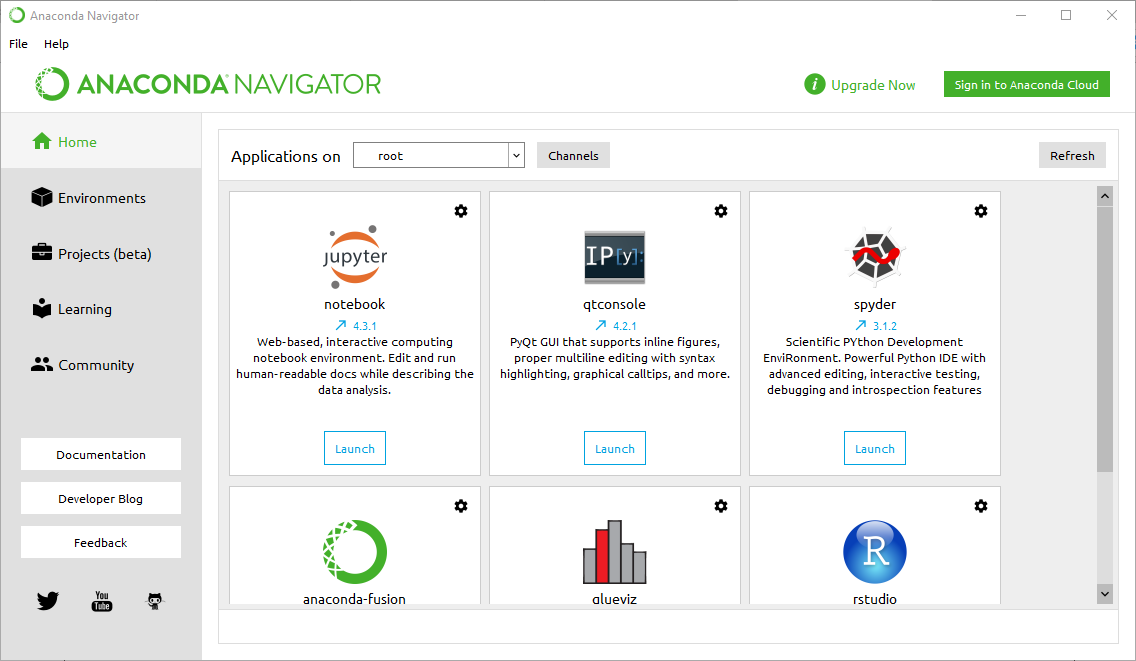
\includegraphics[width=0.7\linewidth]{imgs/AnacondaNavigator.png}}
  \caption{
  Interface graphique du navigateur Anaconda sous Windows
  }
\end{figure}
%\clearpage % flush figures 


Anaconda installe plusieurs exécutables pour développer en Python dans le répertoire \emph{anaconda/bin}, sans toujours créer des raccourcis sur le bureau ou dans un menu. Vous pouvez lancer \textbf{Spyder} ou le notebook \textbf{Jupyter} depuis le navigateur Anaconda.

\subsection{Spyder}
Pour le développement de programmes en langage Python, des applications spéciales appelées IDE (Integrated Development Environment) peuvent être utilisées. Les IDE les plus avancés ont des éditeurs, des consoles, des outils pour organiser des suites de programmes et de bibliothèques, un correcteur orthographique (spell-checking) et une complétion automatiques (auto-completion) pour les scripts partiellement écrits (ces outils connaissent la syntaxe du langage de programmation) et des outils de débogage.

Utiliser un bon éditeur pour programmer en Python est bon. Utiliser un vrai IDE est encore plus confortable et puissant. \textbf{Spyder} (Scientific PYthon Development EnviRonment) semble actuellement très répandu pour l’utilisation scientifique de Python.

Spyder est un environnement de développement interactif gratuit inclus avec Anaconda. Il comprend des fonctionnalités d'édition, de test interactif, de débogage et d'introspection.

Après avoir installé Anaconda, vous pouvez démarrer Spyder sur macOS, Linux ou Windows en ouvrant une fenêtre de terminal (Ubuntu/macOS) ou d'invite de commande (Windows) et en exécutant la commande \texttt{spyder}.


\begin{figure}[!ht]  % 
  \centerline{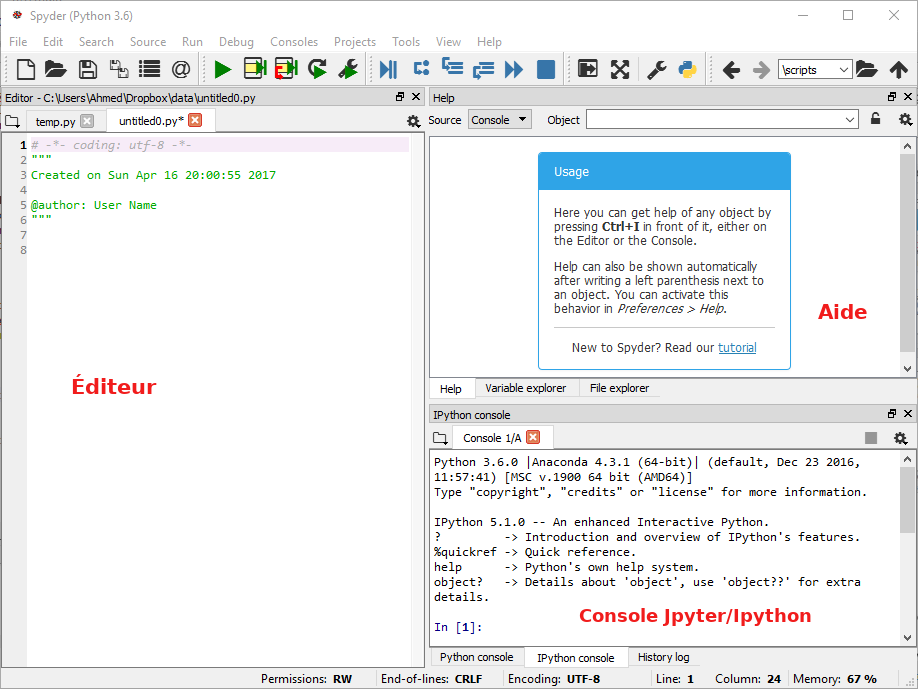
\includegraphics[width=0.7\linewidth]{imgs/SpyderIDE.png}}
  \caption{
  Spyder sous Windows.
  }
\end{figure}
%\clearpage % flush figures 


% !split
\section{Bibliothèques Python largement utilisées}
\subsection{Bibliothèque numérique: \texttt{numpy} }
\textbf{numpy} (\href{{http://www.numpy.org}}{\nolinkurl{http://www.numpy.org}}): Tous les codes numériques Python actuels sont basés sur la bibliothèque \texttt{numpy}. La bibliothèque \texttt{numpy} fournit des structures de données permettant de représenter une grande variété de tableaux, ainsi que des méthodes et des fonctions permettant de fonctionner sur de tels tableaux. \texttt{numpy} fournit le \emph{back-end} numérique pour presque toutes les bibliothèques scientifiques ou techniques de Python. C'est donc une partie très importante de l'écosystème scientifique Python.

\paragraph{Création de tableaux numpy.}
Il existe un certain nombre de façons d’initialiser de nouveaux tableaux numpy, par exemple à partir de:

\begin{itemize}
\item liste ou tuple Python.

\item en utilisant des fonctions dédiées à la génération de tableaux numpy, tels que \texttt{arange}, \texttt{linspace}, etc.

\item lire des données à partir de fichiers.
\end{itemize}

\noindent
Par exemple, pour créer de nouveaux tableaux de vecteurs et matrices à partir de listes Python, nous pouvons utiliser la fonction \texttt{numpy.array}.

\begin{cod}{cbg_gray}\begin{minted}[fontsize=\fontsize{9pt}{9pt},linenos=false,mathescape,baselinestretch=1.0,fontfamily=tt,xleftmargin=2mm]{python}
In [1]: from numpy import array # importation
In [2]: v = array([1,2,3,4]) # un vecteur: l'argument de la fonction array est une liste Python
...: v
Out[2]: array([1, 2, 3, 4])

In [3]: M = array([[1, 2], [3, 4]])  # une matrice: l'argument de la fonction array est une liste Python imbriquée
...: M
Out[3]:
array([[1, 2],
      [3, 4]])
\end{minted}
\end{cod}
\noindent

Les objets \texttt{v} et \texttt{M} sont, les deux, du type \texttt{ndarray} fourni par le module \texttt{numpy}.
Nous pouvons vérifier ça par un simple code:

\begin{cod}{cbg_gray}\begin{minted}[fontsize=\fontsize{9pt}{9pt},linenos=false,mathescape,baselinestretch=1.0,fontfamily=tt,xleftmargin=2mm]{python}
In [4]: print("Le type de v est: ", type(v))
Le type de v est: <class 'numpy.ndarray'>
In [5]: print("Le type de M est: ", type(M))
Le type de M est:  <class 'numpy.ndarray'>
\end{minted}
\end{cod}
\noindent

La différence entre les tableaux \texttt{v} et \texttt{M} réside uniquement dans leurs formes. Nous pouvons obtenir des informations sur la \textbf{forme} d'un tableau en utilisant la propriété \texttt{ndarray.shape}.
\begin{cod}{cbg_gray}\begin{minted}[fontsize=\fontsize{9pt}{9pt},linenos=false,mathescape,baselinestretch=1.0,fontfamily=tt,xleftmargin=2mm]{python}
In [6]: print("La forme de v est: ", v.shape)
La forme de v est:  (4,)
In [7]: print("La forme de M est: ", M.shape)
La forme de M est:  (2, 2)
\end{minted}
\end{cod}
\noindent

\paragraph{Utilisation de fonctions génératrices de tableaux.}
Pour les tableaux de grande taille, il est pratique d'initialiser les données manuellement, en utilisant des listes pythons explicites. Au lieu de cela, nous pouvons utiliser l’une des nombreuses fonctions de \texttt{numpy} qui génère des tableaux de différentes formes.
Certains des plus communs sont:

\begin{itemize}
\item \texttt{arange()}

\item \texttt{linspace()} et \texttt{logspace()}

\item \texttt{mgrid()} et \texttt{meshgrid()}

\item \texttt{diag()}

\item \texttt{zeros()} et \texttt{ones()}

\item etc.
\end{itemize}

\noindent
\paragraph{Fonction \texttt{arange()} :}

\begin{cod}{cbg_gray}\begin{minted}[fontsize=\fontsize{9pt}{9pt},linenos=false,mathescape,baselinestretch=1.0,fontfamily=tt,xleftmargin=2mm]{python}
In [19]: x = arange(0, 10, 1) # Arguments: start, stop, step
    ...: x
Out[19]: array([0, 1, 2, 3, 4, 5, 6, 7, 8, 9])

In [23]: x = arange(-2, 2, 0.1)
    ...: x
Out[23]:
array([-2.00000000e+00, -1.90000000e+00, -1.80000000e+00, -1.70000000e+00,
       -1.60000000e+00, -1.50000000e+00, -1.40000000e+00, -1.30000000e+00,
       -1.20000000e+00, -1.10000000e+00, -1.00000000e+00, -9.00000000e-01,
       -8.00000000e-01, -7.00000000e-01, -6.00000000e-01, -5.00000000e-01,
       -4.00000000e-01, -3.00000000e-01, -2.00000000e-01, -1.00000000e-01,
        1.77635684e-15,  1.00000000e-01,  2.00000000e-01,  3.00000000e-01,
        4.00000000e-01,  5.00000000e-01,  6.00000000e-01,  7.00000000e-01,
        8.00000000e-01,  9.00000000e-01,  1.00000000e+00,  1.10000000e+00,
        1.20000000e+00,  1.30000000e+00,  1.40000000e+00,  1.50000000e+00,
        1.60000000e+00,  1.70000000e+00,  1.80000000e+00,  1.90000000e+00])
\end{minted}
\end{cod}
\noindent

\paragraph{Fonctions \texttt{linspace()} et \texttt{logspace()}:}

En utilisant \texttt{linspace}, les deux points finaux sont inclus:
\begin{cod}{cbg_gray}\begin{minted}[fontsize=\fontsize{9pt}{9pt},linenos=false,mathescape,baselinestretch=1.0,fontfamily=tt,xleftmargin=2mm]{python}
In [24]: linspace(0, 10, 20) # linspace(star, stop, Nombre de points)
Out[24]:
array([ 0.        ,  0.52631579,  1.05263158,  1.57894737,  2.10526316,
        2.63157895,  3.15789474,  3.68421053,  4.21052632,  4.73684211,
        5.26315789,  5.78947368,  6.31578947,  6.84210526,  7.36842105,
        7.89473684,  8.42105263,  8.94736842,  9.47368421, 10.        ])

In [25]: logspace(0, 10, 10, base=e)
Out[25]:
array([1.00000000e+00, 3.03773178e+00, 9.22781435e+00, 2.80316249e+01,
       8.51525577e+01, 2.58670631e+02, 7.85771994e+02, 2.38696456e+03,
       7.25095809e+03, 2.20264658e+04])
\end{minted}
\end{cod}
\noindent

\paragraph{Fonctions \texttt{mgrid()} et \texttt{meshgrid()}:}

\begin{cod}{cbg_gray}\begin{minted}[fontsize=\fontsize{9pt}{9pt},linenos=false,mathescape,baselinestretch=1.0,fontfamily=tt,xleftmargin=2mm]{python}
In [26]: x, y = mgrid[0:5, 0:5] # Similaire à meshgrid dans MATLAB
    ...: x
Out[26]:
array([[0, 0, 0, 0, 0],
       [1, 1, 1, 1, 1],
       [2, 2, 2, 2, 2],
       [3, 3, 3, 3, 3],
       [4, 4, 4, 4, 4]])

In [27]: y
Out[27]:
array([[0, 1, 2, 3, 4],
       [0, 1, 2, 3, 4],
       [0, 1, 2, 3, 4],
       [0, 1, 2, 3, 4],
       [0, 1, 2, 3, 4]])

In [31]: x, y = meshgrid(linspace(0,2,6),linspace(0,2,6))
    ...: x
Out[31]:
array([[0. , 0.4, 0.8, 1.2, 1.6, 2. ],
       [0. , 0.4, 0.8, 1.2, 1.6, 2. ],
       [0. , 0.4, 0.8, 1.2, 1.6, 2. ],
       [0. , 0.4, 0.8, 1.2, 1.6, 2. ],
       [0. , 0.4, 0.8, 1.2, 1.6, 2. ],
       [0. , 0.4, 0.8, 1.2, 1.6, 2. ]])

In [32]: y
Out[32]:
array([[0. , 0. , 0. , 0. , 0. , 0. ],
       [0.4, 0.4, 0.4, 0.4, 0.4, 0.4],
       [0.8, 0.8, 0.8, 0.8, 0.8, 0.8],
       [1.2, 1.2, 1.2, 1.2, 1.2, 1.2],
       [1.6, 1.6, 1.6, 1.6, 1.6, 1.6],
       [2. , 2. , 2. , 2. , 2. , 2. ]])
\end{minted}
\end{cod}
\noindent

\paragraph{Fonctions \texttt{rand()}, \texttt{randint()}:}

Nombres aléatoires uniformes dans [0,1[ dans une matrice (3,2)
\begin{cod}{cbg_gray}\begin{minted}[fontsize=\fontsize{9pt}{9pt},linenos=false,mathescape,baselinestretch=1.0,fontfamily=tt,xleftmargin=2mm]{python}
In [37]: rand(3,2)
Out[37]:
array([[0.01900499, 0.10872428],
       [0.78849226, 0.22114384],
       [0.88739675, 0.94190273]])
\end{minted}
\end{cod}
\noindent

Générer un tableau 2 x 4 d'entiers compris entre 0 et 4 inclus.
\begin{cod}{cbg_gray}\begin{minted}[fontsize=\fontsize{9pt}{9pt},linenos=false,mathescape,baselinestretch=1.0,fontfamily=tt,xleftmargin=2mm]{python}
In [39]: randint(5, size=(2, 4))
Out[39]:
array([[0, 1, 4, 4],
       [4, 0, 0, 4]])
\end{minted}
\end{cod}
\noindent

\paragraph{Fonction \texttt{diag()}:}

\begin{cod}{cbg_gray}\begin{minted}[fontsize=\fontsize{9pt}{9pt},linenos=false,mathescape,baselinestretch=1.0,fontfamily=tt,xleftmargin=2mm]{python}
In [40]: # Une matrice diagonale
    ...: diag([1,2,3])
Out[40]:
array([[1, 0, 0],
       [0, 2, 0],
       [0, 0, 3]])

In [41]: # Diagonale avec décalage de la diagonale principale
    ...: diag([1,2,3], k=3)
Out[41]:
array([[0, 0, 0, 1, 0, 0],
       [0, 0, 0, 0, 2, 0],
       [0, 0, 0, 0, 0, 3],
       [0, 0, 0, 0, 0, 0],
       [0, 0, 0, 0, 0, 0],
       [0, 0, 0, 0, 0, 0]])
\end{minted}
\end{cod}
\noindent

\paragraph{Fonctions \texttt{zeros()} et \texttt{ones()}:}

\begin{cod}{cbg_gray}\begin{minted}[fontsize=\fontsize{9pt}{9pt},linenos=false,mathescape,baselinestretch=1.0,fontfamily=tt,xleftmargin=2mm]{python}
In [42]: zeros((3,3))
Out[42]:
array([[0., 0., 0.],
       [0., 0., 0.],
       [0., 0., 0.]])

In [43]: ones((3,3))
Out[43]:
array([[1., 1., 1.],
       [1., 1., 1.],
       [1., 1., 1.]])
\end{minted}
\end{cod}
\noindent

\paragraph{Lecture et écriture de données.}
\paragraph{Écriture de données}

Le module \texttt{numpy} contient une fonction très pratique, \texttt{savetxt}, permettant d’enregistrer des données tabulaires. Les données doivent être stockées dans un tableau numpy à deux dimensions. La fonction \texttt{savetxt} permet de contrôler le format des nombres dans chaque colonne (\texttt{fmt}), un en-tête peut être ajouté (\texttt{header}) et les lignes d'en-tête commencent par un caractère de commentaire (\texttt{comment}).


\begin{block_grayiconadmon}[Exemple]

Pour stoker les valeurs de $cos(x)$ avec $x \in [0, 2 \pi]$ dans un fichier \emph{cosinus.dat}, le code est comme ci-dessous:

\begin{cod}{cbg_gray}\begin{minted}[fontsize=\fontsize{9pt}{9pt},linenos=false,mathescape,baselinestretch=1.0,fontfamily=tt,xleftmargin=2mm]{python}
'''Créer un tableau à deux dimensions de
[x, cos (x)] dans chaque ligne'''
import numpy as np
x = np.linspace(0, 2*np.pi, 200) # 200 valeurs de x
# un tableau 2 colonnes 200 lignes
data = np.array([x, np.cos(x)]).transpose()

# Écrire un tableau de données dans un fichier sous forme de tableau
np.savetxt('cosinus.dat', data, fmt=['%.2f', '%.4f'],
           header='x   cos(x)', comments='#')
\end{minted}
\end{cod}
\noindent
Le fichier \emph{cosinus.dat} est créé dans le répertoire de travail:
\begin{cod}{cbg_gray}\begin{minted}[fontsize=\fontsize{9pt}{9pt},linenos=false,mathescape,baselinestretch=1.0,fontfamily=tt,xleftmargin=2mm]{text}
# x   cos(x)
0.00 1.0000
0.03 0.9995
0.06 0.9980
0.09 0.9955
0.13 0.9920
0.16 0.9876
0.19 0.9821
0.22 0.9757
0.25 0.9683
...  ......
...  ......
\end{minted}
\end{cod}
\noindent
\end{block_grayiconadmon} % title: Exemple



\paragraph{Lecture de données}

Les données du fichier \emph{cosinus.dat} peuvent être lues dans un tableau \texttt{numpy} par la fonction \texttt{loadtxt} (vous pouvez utiliser la commande \texttt{help(loadtxt)} dans le notebook pour comprendre l'utilité des arguments entre les parenthèse):

\begin{cod}{cbg_gray}\begin{minted}[fontsize=\fontsize{9pt}{9pt},linenos=false,mathescape,baselinestretch=1.0,fontfamily=tt,xleftmargin=2mm]{python}

In [51]: data = np.loadtxt('cosinus.dat', comments='#')
    ...: data
Out[51]:
array([[ 0.    ,  1.    ],
       [ 0.03  ,  0.9995],
       [ 0.06  ,  0.998 ],
       [ 0.09  ,  0.9955],
       [ 0.13  ,  0.992 ],
       [ 0.16  ,  0.9876],
       [ 0.19  ,  0.9821],
       [ 0.22  ,  0.9757],
       [ 0.25  ,  0.9683],
       [ 0.28  ,  0.9599],
       ..................
       ..................
       ..................
       [ 6.22  ,  0.998 ],
       [ 6.25  ,  0.9995],
       [ 6.28  ,  1.    ]])
\end{minted}
\end{cod}
\noindent


\begin{notice_grayiconadmon}[Notice]
Les lignes commençant par le caractère de commentaire sont ignorées lors de la lecture. L'objet \texttt{data} résultant est un tableau à deux dimensions: \texttt{data[i, j]} contient le numéro de ligne \texttt{i} et le numéro de colonne \texttt{j} dans la table, c'est-à-dire que \texttt{data[i, 0]} contiennent la valeur \texttt{x} et que \texttt{data[i, 1]} la valeur \texttt{cos(x)} dans la i-ème ligne.
\end{notice_grayiconadmon} % title: Notice



Nous pouvons utiliser le fichier \emph{cosinus.dat} pour tracer la fonction $cos(x)$ comme indiqué dans le code suivant:

\begin{cod}{cbg_gray}\begin{minted}[fontsize=\fontsize{9pt}{9pt},linenos=false,mathescape,baselinestretch=1.0,fontfamily=tt,xleftmargin=2mm]{python}
import numpy as np
import matplotlib.pyplot as plt
# Charger les données du fichier 'cosinus.dat'
X, C = np.loadtxt('cosinus.dat', comments='#', unpack=True)
# Tracer C en fonction de X
plt.figure(figsize=(8, 5), dpi=100)
plt.plot(X,C)
plt.savefig("fonct_trig4.png")
plt.savefig("fonct_trig4.pdf")
plt.show()
\end{minted}
\end{cod}
\noindent

La sortie de ce code est la Figure~\ref{figout:trig4}.

\begin{figure}[!ht]  % figout:trig4
  \centerline{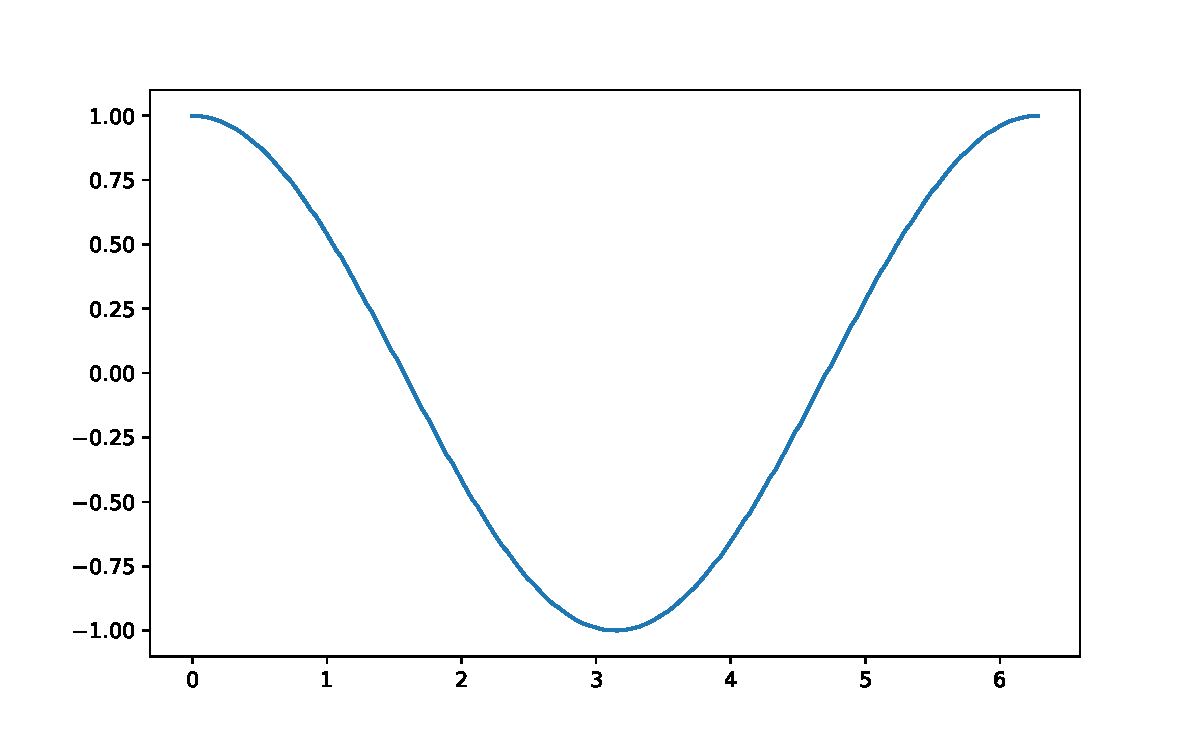
\includegraphics[width=0.7\linewidth]{imgs/fonct_trig4.pdf}}
  \caption{
  Fonction trigonométrique, $cos(x)$, générée à partir d'un fichier. \label{figout:trig4}
  }
\end{figure}
%\clearpage % flush figures figout:trig4


% !split
\subsection{Bibliothèque Python de visualisation des données: \texttt{matplotlib} }
\texttt{matplotlib} (\href{{http://matplotlib.org/}}{\nolinkurl{http://matplotlib.org/}}) est une excellente bibliothèque graphique 2D et 3D pour générer des graphiques scientifiques. Voici quelques-uns des nombreux avantages de cette bibliothèque:

\begin{itemize}
\item Facile à utiliser

\item Prise en charge des étiquettes et des textes formatés {\LaTeX}

\item Un excellent contrôle des éléments d'une figure, y compris la taille et la résolution (DPI).

\item Sortie de haute qualité dans de nombreux formats, y compris PNG, PDF, SVG, EPS, ...

\item GUI (Graphical User Interface) pour explorer interactivement les figures.
\end{itemize}

\noindent
\paragraph{Documentation en ligne et Galerie.}
Vous trouverez plus d'informations, y compris une documentation complète avec une vaste galerie d'exemples, sur le site de \texttt{mtplotlib}.

De nombreux utilisateurs de \texttt{matplotlib} sont souvent confrontés à la question:

\begin{quote}
Je veux tracer les courbes de deux fonctions ($f$ te $g$) \textbf{ressemblant} à une troisième ($h$)?
\end{quote}

 Je souhaite bonne chance à ceux qui désirent obtenir rapidement une réponse, même avec l'aide de \textbf{google}!. C'est pourquoi la \textbf{galerie de matplotlib} (\href{{http://matplotlib.org/gallery.html}}{\nolinkurl{http://matplotlib.org/gallery.html}}) est si utile, car elle montre la variété des possibilités. Ainsi, vous pouvez parcourir la galerie, cliquer sur n'importe quel graphique qui comporte les éléments que vous voulez reproduire et afficher le code qui a servi à le générer. Vous deviendrez rapidement autonome, vous allez mélanger et assortir différents composants pour produire votre propre chef-d’œuvre!

\paragraph{Guide de Démarrage}
L'exemple ci-dessous montre comment, de manière très simple, représenter graphiquement la fonction $f(x) = y = x$.
\begin{pro}{cbg_gray}{bar_gray}\begin{minted}[fontsize=\fontsize{9pt}{9pt},linenos=false,mathescape,baselinestretch=1.0,fontfamily=tt,xleftmargin=2mm]{python}
# -*- coding: utf-8 -*-
# importaion
import matplotlib.pyplot as plt
# define x
x = [1, 3, 5, 6, 8, 10, 15]
# define y
y=x
# créer un nouveau graphique
plt.figure()
#plot f(x)= x
plt.plot(x, y)
# Écrire un texte (label) sur l'axe des x
plt.xlabel("X-Axis")
# Écrire un texte (label) sur l'axe des y
plt.ylabel("Y-Axis")
#les graphiques ne seront affichés que lorsque vous appelez plt.show ()
plt.show()
\end{minted}
\end{pro}
\noindent


\begin{figure}[!ht]  % fig:BasicPlot1
  \centerline{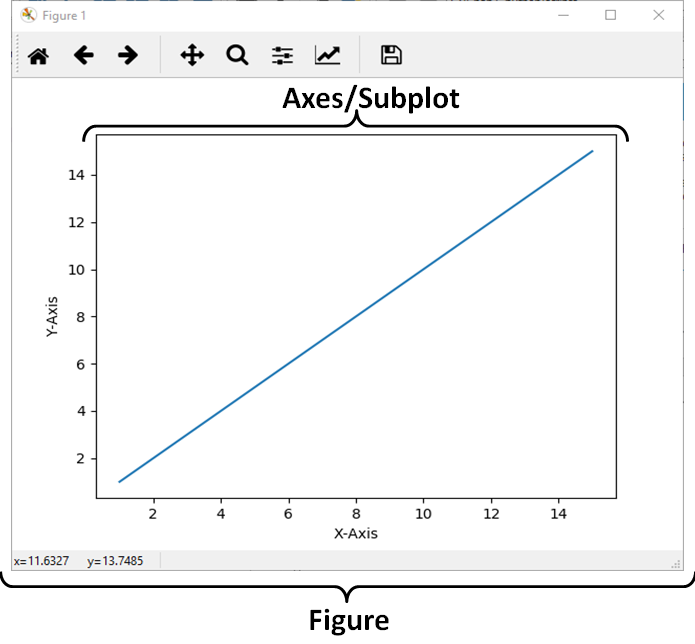
\includegraphics[width=0.7\linewidth]{imgs/BasicPlot1.png}}
  \caption{
  Fenêtre de traçage de matplotlib. \label{fig:BasicPlot1}
  }
\end{figure}
%\clearpage % flush figures fig:BasicPlot1


Le graphique (\texttt{Figure}) est le conteneur de niveau supérieur dans cette hiérarchie. C'est la fenêtre/page globale sur laquelle tout est dessiné.
Vous pouvez avoir plusieurs figures indépendantes et les graphiques peuvent contenir plusieurs \texttt{Axes}.

La plupart des tracés ont lieu sur des \texttt{Axes}. C’est effectivement la zone sur laquelle nous traçons les données et les graduations/labels/etc. qui leur sont associés. Habituellement, nous configurons un \texttt{Axes} avec un appel à \texttt{Subplot} (qui place les \texttt{Axes} sur une grille régulière). Par conséquent, dans la plupart des cas, \texttt{Axes} et \texttt{Subplot} sont synonymes (figure). Chaque \texttt{Axes} ou \texttt{Subplot} a un axe X et un axe Y. Ceux-ci contiennent les graduations, les emplacements de graduations, etc.

\paragraph{Vues en grille }
Nous avons déjà mentionné qu’une figure peut avoir plus d’un axe. Si vous voulez que vos axes soient sur un système de grille standard, il est alors plus simple d'utiliser \texttt{plt.subplot(...)} pour créer un graphique et y ajouter les axes automatiquement.
\begin{pro}{cbg_gray}{bar_gray}\begin{minted}[fontsize=\fontsize{9pt}{9pt},linenos=false,mathescape,baselinestretch=1.0,fontfamily=tt,xleftmargin=2mm]{python}
# -*- coding: utf-8 -*-
import matplotlib.pyplot as plt
fig1=plt.figure(1)                # the first figure
ax1=plt.subplot(211)             # the first subplot in the first figure
ax1.plot([1, 2, 3])
ax2=plt.subplot(212)             # the second subplot in the first figure
ax2.plot([4, 5, 6])

fig2=plt.figure(2)                # a second figure
plt.plot([4, 5, 6])          # creates a subplot(111) by default

fig1=plt.figure(1)                # figure 1 current; subplot(212) still current
ax1=plt.subplot(211)             # make subplot(211) in figure1 current
ax1.set_title('Easy as 1, 2, 3') # subplot 211 title
plt.show()
\end{minted}
\end{pro}
\noindent


\begin{figure}[!ht]  % fig:subplot1
  \centerline{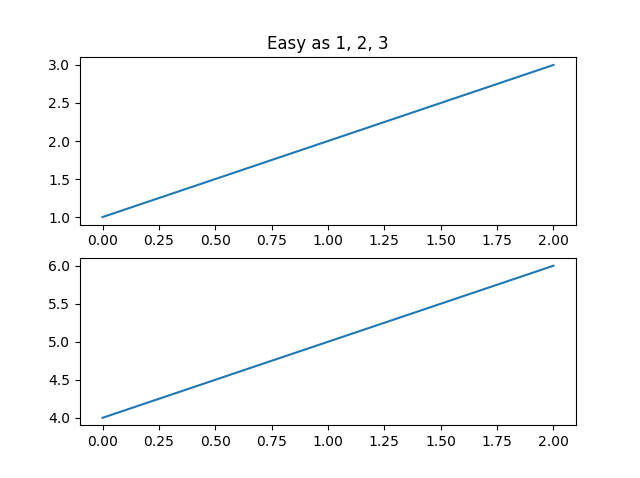
\includegraphics[width=0.7\linewidth]{imgs/subplot1.png}}
  \caption{
  Vue en grille, figure(1). \label{fig:subplot1}
  }
\end{figure}
%\clearpage % flush figures fig:subplot1



\begin{figure}[!ht]  % fig:subplot2
  \centerline{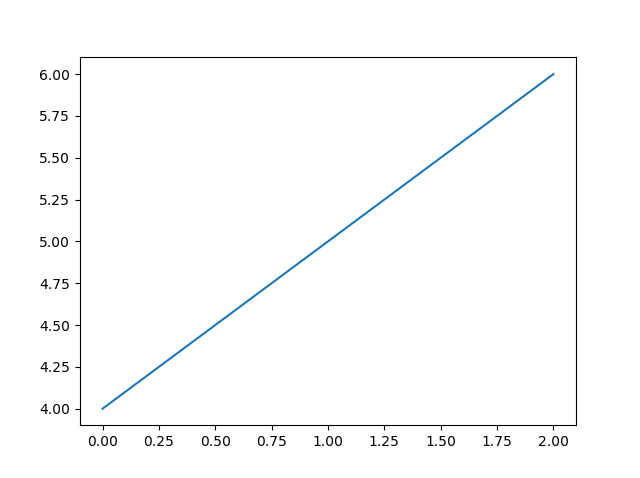
\includegraphics[width=0.7\linewidth]{imgs/subplot2.png}}
  \caption{
  Graphique unique, figure(2). \label{fig:subplot2}
  }
\end{figure}
%\clearpage % flush figures fig:subplot2


\paragraph{Commandes de texte de base}
Les commandes suivantes permettent de créer du texte dans l'interface \texttt{pyplot}:
\begin{itemize}
\item \texttt{text()} - ajoute du texte à un emplacement quelconque sur les axes; \texttt{matplotlib.axes.Axes.text()}.

\item \texttt{xlabel()} - ajoute une étiquette à l'axe des x; \Verb!matplotlib.axes.Axes.set_xlabel()!

\item \texttt{ylabel()} - ajoute une étiquette à l'axe des y; \Verb!matplotlib.axes.Axes.set_ylabel()!

\item \texttt{title()} - ajoute un titre aux Axes; \Verb!matplotlib.axes.Axes.set_title()!

\item \texttt{figtext()} - ajoute du texte à un emplacement quelconque sur la figure; \texttt{matplotlib.figure.Figure.text()}

\item \texttt{suptitle()} - ajoute un titre à la figure; \texttt{matplotlib.figure.Figure.suptitle()}

\item \texttt{annotate()} - ajoute une annotation, avec une flèche optionnelle, aux axes; \texttt{matplotlib.axes.Axes.annotate()}
\end{itemize}

\noindent
Toutes ces fonctions créent et renvoient une instance \texttt{matplotlib.text.Text()}, qui peut être configurée avec diverses polices et autres propriétés. L'exemple ci-dessous montre toutes ces commandes en action.

\begin{pro}{cbg_gray}{bar_gray}\begin{minted}[fontsize=\fontsize{9pt}{9pt},linenos=false,mathescape,baselinestretch=1.0,fontfamily=tt,xleftmargin=2mm]{python}
# -*- coding: utf-8 -*-
import matplotlib.pyplot as plt

fig = plt.figure()
fig.suptitle('bold figure suptitle', fontsize=14, fontweight='bold')

ax = fig.add_subplot(111)
fig.subplots_adjust(top=0.85)
ax.set_title('axes title')

ax.set_xlabel('xlabel')
ax.set_ylabel('ylabel')

ax.text(3, 8, 'boxed italics text in data coords', style='italic',
        bbox={'facecolor':'red', 'alpha':0.5, 'pad':10})

ax.text(2, 6, r'an equation: $E=mc^2$', fontsize=15)

ax.text(3, 2, u'unicode: Institut f\374r Festk\366rperphysik')

ax.text(0.95, 0.01, 'colored text in axes coords',
        verticalalignment='bottom', horizontalalignment='right',
        transform=ax.transAxes,
        color='green', fontsize=15)


ax.plot([2], [1], 'o')
ax.annotate('annotate', xy=(2, 1), xytext=(3, 4),
            arrowprops=dict(facecolor='black', shrink=0.05))

ax.axis([0, 10, 0, 10])

plt.show()
\end{minted}
\end{pro}
\noindent


\begin{figure}[!ht]  % fig:BasicText
  \centerline{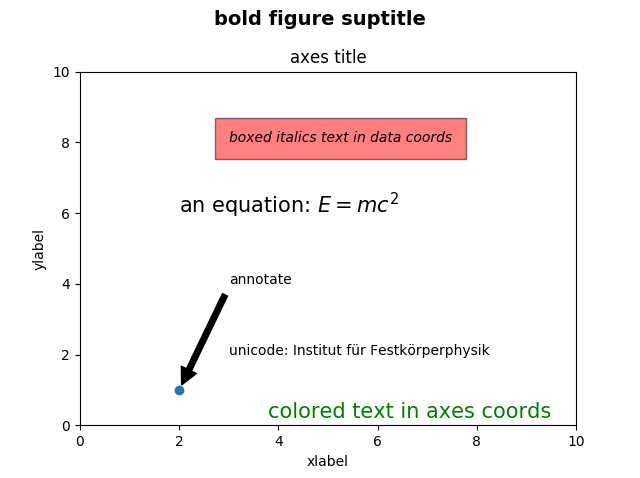
\includegraphics[width=0.7\linewidth]{imgs/BasicText.png}}
  \caption{
  Texte de base. \label{fig:BasicText}
  }
\end{figure}
%\clearpage % flush figures fig:BasicText


\paragraph{Styles de lignes et de marqueurs}
Pour changer la largeur de ligne, nous pouvons utiliser l'argument de mot-clé \texttt{linewidth} ou \texttt{lw}, et le style de ligne peut être sélectionné à l'aide des arguments de mot-clé \texttt{linestyle} ou \texttt{ls}:

\begin{pro}{cbg_gray}{bar_gray}\begin{minted}[fontsize=\fontsize{9pt}{9pt},linenos=false,mathescape,baselinestretch=1.0,fontfamily=tt,xleftmargin=2mm]{python}
# -*- coding: utf-8 -*-
import matplotlib.pyplot as plt
import numpy as np
x = np.linspace(0, 5, 10)
fig, ax = plt.subplots()

ax.plot(x, x+1, color="blue", linewidth=0.25)
ax.plot(x, x+2, color="blue", linewidth=0.50)
ax.plot(x, x+3, color="blue", linewidth=1.00)
ax.plot(x, x+4, color="blue", linewidth=2.00)

# possible linestype options '-', '-.', ':', 'steps'
ax.plot(x, x+5, color="red", lw=2, linestyle='-')
ax.plot(x, x+6, color="red", lw=2, ls='-.')
ax.plot(x, x+7, color="red", lw=2, ls=':')

# custom dash
line, = ax.plot(x, x+8, color="black", lw=1.50)
line.set_dashes([5, 10, 15, 10]) # format: line length, space length, ...

# possible marker symbols: marker = '+', 'o', '*', 's', ',', '.', '1', '2', '3', '4', ...
ax.plot(x, x+ 9, color="green", lw=2, ls='-.', marker='+')
ax.plot(x, x+10, color="green", lw=2, ls='-.', marker='o')
ax.plot(x, x+11, color="green", lw=2, ls='-.', marker='s')
ax.plot(x, x+12, color="green", lw=2, ls='-.', marker='1')

# marker size and color
ax.plot(x, x+13, color="purple", lw=1, ls='-', marker='o', markersize=2)
ax.plot(x, x+14, color="purple", lw=1, ls='-', marker='o', markersize=4)
ax.plot(x, x+15, color="purple", lw=1, ls='-', marker='o', markersize=8, markerfacecolor="red")
ax.plot(x, x+16, color="purple", lw=1, ls='-', marker='s', markersize=8, 
        markerfacecolor="yellow", markeredgewidth=2, markeredgecolor="blue")
# make a title for the subplot
ax.set_title('"ax.plot(x, y, ...)": Lines and/or markers', fontsize=16, weight='bold')
# make x and y axis label and set their font size and weight
ax.set_xlabel("X-Axis", fontsize=12, weight='bold')
ax.set_ylabel("Y-Axis", fontsize=12, weight='bold')
plt.show()
\end{minted}
\end{pro}
\noindent


\begin{figure}[!ht]  % fig:LineandMarkerStyles
  \centerline{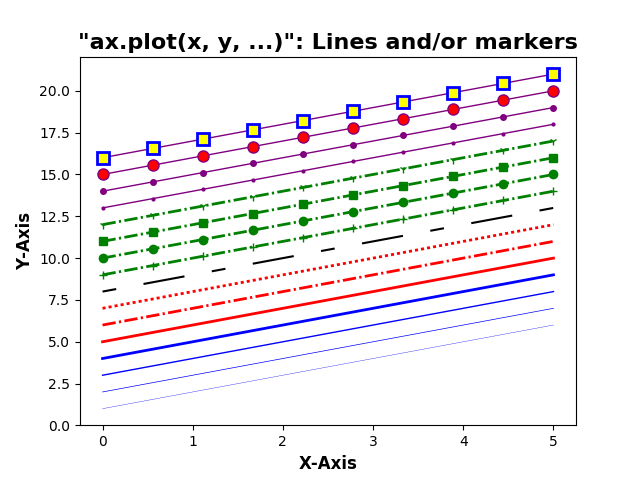
\includegraphics[width=0.7\linewidth]{imgs/LineandMarkerStyles.png}}
  \caption{
  Styles de lignes et de marqueurs. \label{fig:LineandMarkerStyles}
  }
\end{figure}
%\clearpage % flush figures fig:LineandMarkerStyles


\paragraph{Colormap: Tracés contour, Imshow et 33D}


Voir la documentation de matplotlib colormaps \href{{http://matplotlib.org/users/colormaps.html}}{\nolinkurl{http://matplotlib.org/users/colormaps.html}}.

\begin{itemize}
 \item \textbf{Tracés contour :}
\end{itemize}

\noindent
\begin{pro}{cbg_gray}{bar_gray}\begin{minted}[fontsize=\fontsize{9pt}{9pt},linenos=false,mathescape,baselinestretch=1.0,fontfamily=tt,xleftmargin=2mm]{python}
# -*- coding: utf-8 -*-
import numpy as np
import matplotlib.pyplot as plt

def f(x,y):
    return (1 - x / 2 + x**5 + y**3) * np.exp(-x**2 -y**2)

n = 256
x = np.linspace(-3, 3, n)
y = np.linspace(-3, 3, n)
X,Y = np.meshgrid(x, y)

plt.axes([0.025, 0.025, 0.95, 0.95])

plt.contourf(X, Y, f(X, Y), 8, alpha=.75, cmap=plt.cm.gray)
C = plt.contour(X, Y, f(X, Y), 8, colors='black', linewidth=.5)
plt.clabel(C, inline=1, fontsize=10)

plt.xticks(())
plt.yticks(())
plt.show()
\end{minted}
\end{pro}
\noindent


\begin{figure}[!ht]  % fig:ContourPlot
  \centerline{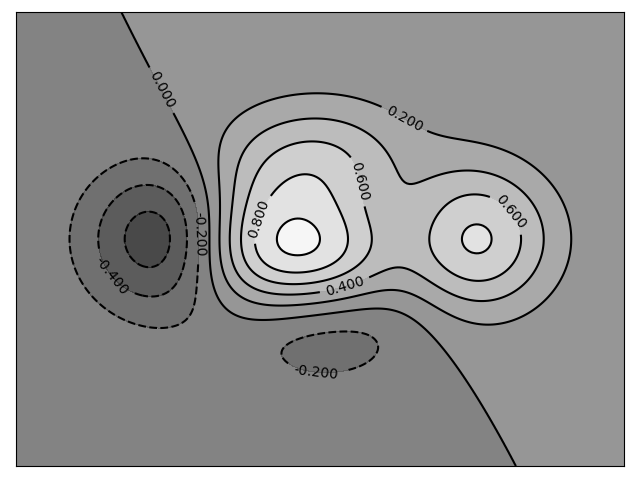
\includegraphics[width=0.7\linewidth]{imgs/ContourPlot.png}}
  \caption{
  Exemple de tracé de contour. \label{fig:ContourPlot}
  }
\end{figure}
%\clearpage % flush figures fig:ContourPlot


\begin{itemize}
\item \textbf{Imshow (Image pixelisée) :}
\end{itemize}

\noindent
\begin{pro}{cbg_gray}{bar_gray}\begin{minted}[fontsize=\fontsize{9pt}{9pt},linenos=false,mathescape,baselinestretch=1.0,fontfamily=tt,xleftmargin=2mm]{python}
# -*- coding: utf-8 -*-
import numpy as np
import matplotlib.pyplot as plt

def f(x, y):
    return (1 - x / 2 + x ** 5 + y ** 3 ) * np.exp(-x ** 2 - y ** 2)

n = 10
x = np.linspace(-3, 3, 3.5 * n)
y = np.linspace(-3, 3, 3.0 * n)
X, Y = np.meshgrid(x, y)
Z = f(X, Y)

plt.axes([0.025, 0.025, 0.95, 0.95])
plt.imshow(Z, interpolation='nearest', cmap='gray', origin='lower')
plt.colorbar(shrink=.92)

plt.xticks(())
plt.yticks(())
plt.show()
\end{minted}
\end{pro}
\noindent


\begin{figure}[!ht]  % fig:CImshow
  \centerline{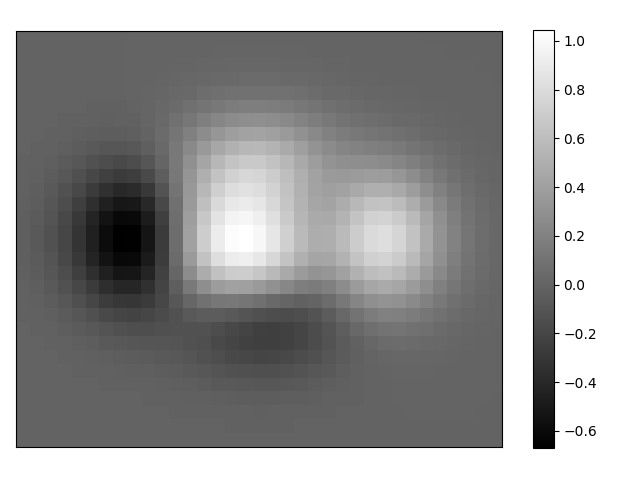
\includegraphics[width=0.7\linewidth]{imgs/Imshow.png}}
  \caption{
  Exemple d'image pixelisée. \label{fig:CImshow}
  }
\end{figure}
%\clearpage % flush figures fig:CImshow


\begin{itemize}
\item \textbf{Tracé en 3D :}
\end{itemize}

\noindent
\begin{pro}{cbg_gray}{bar_gray}\begin{minted}[fontsize=\fontsize{9pt}{9pt},linenos=false,mathescape,baselinestretch=1.0,fontfamily=tt,xleftmargin=2mm]{python}
# -*- coding: utf-8 -*-
import numpy as np
import matplotlib.pyplot as plt
from mpl_toolkits.mplot3d import Axes3D

fig = plt.figure()
ax = Axes3D(fig)
X = np.arange(-4, 4, 0.25)
Y = np.arange(-4, 4, 0.25)
X, Y = np.meshgrid(X, Y)
R = np.sqrt(X ** 2 + Y ** 2)
Z = np.sin(R)

ax.plot_surface(X, Y, Z, rstride=1, cstride=1, cmap=plt.cm.gray)
ax.contourf(X, Y, Z, zdir='z', offset=-2, cmap=plt.cm.gray)
ax.set_zlim(-2, 2)

plt.show()
\end{minted}
\end{pro}
\noindent


\begin{figure}[!ht]  % fig:3D
  \centerline{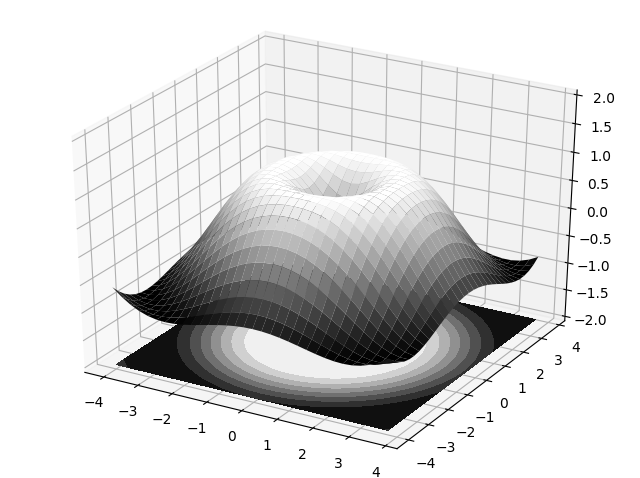
\includegraphics[width=0.7\linewidth]{imgs/Plot3D.png}}
  \caption{
  Exemple de tracé en 3D. \label{fig:3D}
  }
\end{figure}
%\clearpage % flush figures fig:3D


% !split
\subsection{Bibliothèque scientifique python: \texttt{scipy} }
\texttt{scipy} (\href{{https://www.scipy.org/}}{\nolinkurl{https://www.scipy.org/}}"): \texttt{scipy} peut être considéré comme une extension de \texttt{numpy} avec un grand nombre de modules optimisés pour des calculs scientifiques spécifiques. \texttt{scipy} est la plate-forme la plus importante de Python pour le calcul scientifique. La communauté de \texttt{scipy} est un groupe bien établi et en pleine croissance de scientifiques, d’ingénieurs et de chercheurs qui utilisent, développent et promeuvent l’utilisation de Python pour le calcul scientifique, la recherche et l’éducation.

\paragraph{Fonctions spéciales.}
Un grand nombre de fonctions mathématiques spéciales sont importantes pour de nombreux problèmes de physique informatique. SciPy fournit des implémentations d'un ensemble très complet de fonctions spéciales. Pour plus de détails, voir la liste des fonctions dans la documentation de référence à \href{{http://docs.scipy.org/doc/scipy/reference/special.html#module-scipy.special}}{\nolinkurl{http://docs.scipy.org/doc/scipy/reference/special.html\#module-scipy.special}}.

\paragraph{Fonctions de Bessel}

Le module \texttt{scipy.special} inclut un grand nombre de fonctions de Bessel. Ici, nous allons utiliser les fonctions \texttt{jn} et \texttt{yn}, qui sont les fonctions de Bessel des premier et deuxième ordres de type et de valeurs réelles. Nous incluons également la fonction \Verb!jn_zeros! et \Verb!yn_zeros! qui donne les zéros des fonctions \texttt{jn} et \texttt{yn}.

\begin{pro}{cbg_gray}{bar_gray}\begin{minted}[fontsize=\fontsize{9pt}{9pt},linenos=false,mathescape,baselinestretch=1.0,fontfamily=tt,xleftmargin=2mm]{python}
# -*- coding: utf-8 -*-
from scipy.special import jn, yn, jn_zeros, yn_zeros
import matplotlib.pyplot as plt
import numpy as np

n = 0    # order
x = 0.0

# Bessel function of first kind
print ("J_%d(%f) = %f" % (n, x, jn(n, x)))

x = 1.0
# Bessel function of second kind
print ("Y_%d(%f) = %f" % (n, x, yn(n, x)))

# zeros of Bessel functions
n = 0 # order
m = 4 # number of roots to compute
print("zeros of Bessel functions are: ", jn_zeros(n, m))

# Plot Bessel fonctions
x = np.linspace(0, 10, 50)

markers=['o', 's', '*', '+']
lines=['-', '--', '-.', ':']

fig, ax = plt.subplots()
for n in range(4):
    ax.plot(x, jn(n, x),ls=str(lines[n]),marker=str(markers[n]), label=r"$J_%d(x)$" % n)
ax.legend()
plt.show()
\end{minted}
\end{pro}
\noindent

Ce code retournera:
\begin{cod}{cbg_gray}\begin{minted}[fontsize=\fontsize{9pt}{9pt},linenos=false,mathescape,baselinestretch=1.0,fontfamily=tt,xleftmargin=2mm]{text}
J_0(0.000000) = 1.000000
Y_0(1.000000) = 0.088257
zeros of Bessel functions are:  [  2.40482556   5.52007811   8.65372791  11.79153444]
\end{minted}
\end{cod}
\noindent

et le tracé:


\begin{figure}[!ht]  % fig:Bessel
  \centerline{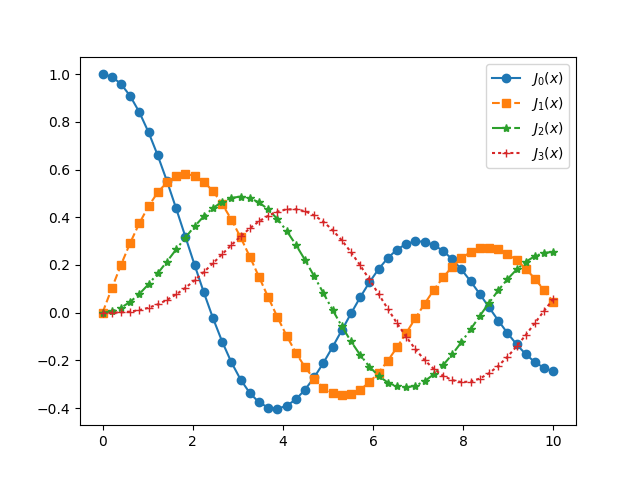
\includegraphics[width=0.7\linewidth]{imgs/Bessel.png}}
  \caption{
  Fonctions de Bessel. \label{fig:Bessel}
  }
\end{figure}
%\clearpage % flush figures fig:Bessel


\paragraph{Intégrales de Fresnel}

La fonction \texttt{scipy.special.fresnel} renvoie les deux fonctions de Fresnel mais dans l'ordre (FS, FC), où FS représente l'intégrale de sinus de Fresnel et FC, l'intégrale de cosinus de Fresnel. Vous devriez faire attention à ce que vos tracés correspondent à la spirale de Cornu.

\begin{pro}{cbg_gray}{bar_gray}\begin{minted}[fontsize=\fontsize{9pt}{9pt},linenos=false,mathescape,baselinestretch=1.0,fontfamily=tt,xleftmargin=2mm]{python}
# -*- coding: utf-8 -*-
from scipy.special import fresnel
from scipy import linspace
import matplotlib.pyplot as plt
t = linspace(-10, 10, 1000)
FS, FC = fresnel(t)
fig1=plt.figure(figsize=(10,5))
ax1=plt.subplot(1, 2, 1)
ax1.plot(FC, FS, linewidth=2)
ax1.set_xlabel("C(t)", fontsize=14, weight='bold')
ax1.set_ylabel("S(t)", fontsize=14, weight='bold')
ax1.set_title("Cornu spiral", fontsize=16, weight='bold')

ax2=plt.subplot(1, 2, 2) 
ax2.plot(t, FS, ls='--',linewidth=2,label="S(t)", alpha=.8)
ax2.plot(t, FC,ls='-',linewidth=2,label="C(t)", alpha=.8)
ax2.set_xlabel("t", fontsize=14, weight='bold')
ax2.set_title("Fresnel integrals", fontsize=16, weight='bold')
plt.legend()
plt.show()
\end{minted}
\end{pro}
\noindent


\begin{figure}[!ht]  % fig:Fresnel
  \centerline{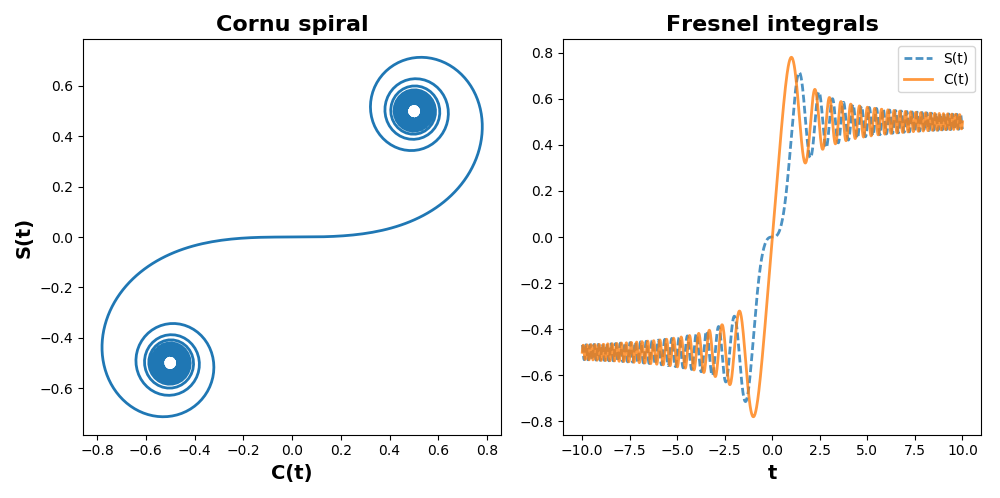
\includegraphics[width=0.7\linewidth]{imgs/Fresnel.png}}
  \caption{
  Intégrales de Fresnel. \label{fig:Fresnel}
  }
\end{figure}
%\clearpage % flush figures fig:Fresnel


% ------------------- end of main content ---------------

% #ifdef PREAMBLE
\end{document}
% #endif

